\section{VCVS Voltage Gain}

\subsection{VCVS Voltage Gain}
\begin{frame}{Pengantar VCVS Voltage Gain}
	\begin{itemize}
		\item Sebelumnya kita telah menganalisa noninverting amplifier, sebuah implementasi secara luas dari VCVS.
		\item Pada bab ini, kita akan memeriksa kembali noninverting amplifier dan menggali lebih dalam terkait voltage gain-nya.
	\end{itemize}
\end{frame}

\subsection{Exact Closed-Loop Voltage Gain}
\begin{frame}{Exact Closed-Loop Voltage Gain}
	\begin{figure}
		\centering
		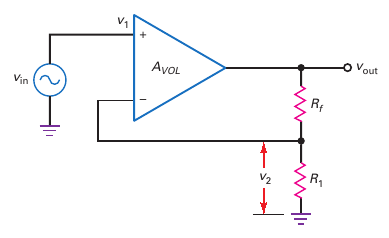
\includegraphics[height=0.7\textheight]{gambar/fig-17.03}
		\caption{VCVS amplifier / noninverting amplifier}
		\label{fig-17.03}
	\end{figure}
\end{frame}


\begin{frame}{Exact Closed-Loop Voltage Gain}
	\begin{itemize}
		\item Sebuah op amp biasanya memiliki open-loop voltage gain ($ A_{VOL} $) sebesar 100000 bahkan lebih.
		\item Karena ada pembagi tegangan maka sebagian dari tegangan output diumpankan kembali ke inverting input.
		\item Feedback fraction atau feedback attenuation factor: mengindikasikan berapa banyak tegangan keluaran teratenuasi sebelum sinyal feedback mencapai inverting input.
		\item Persamaan feedback fraction adalah
		\begin{equation}\label{pers-17.01}
			B = \frac{v_2}{v_{out}}
		\end{equation}
	\end{itemize}
\end{frame}

\begin{frame}{Exact Closed-Loop Voltage Gain}
	\begin{itemize}
		\item Closed-loop voltage gain:
		\begin{equation}\label{pers-17.02}
			A_{v(CL)} = \frac{A_{VOL}}{1 + A_{VOL}B}
		\end{equation}
		\item Berdasarkan Gambar \ref{tabel-17.1}, $ A_v = A_{v(CL)} $, maka exact closed-loop voltage gain dari setiap VCVS:
		\begin{equation}\label{pers-17.03}
			A_v = \frac{A_{VOL}}{1 + A_{VOL}B}
		\end{equation}
	\end{itemize}
\end{frame}

\subsection{Loop Gain}
\begin{frame}{Loop Gain}
	\begin{itemize}
		\item Istilah dari $ A_{VOL} B$ adalah Loop Gain.
		\item Disebut loop gain karena voltage gain dari forward dan feedback path.
		\item Loop gain sangat penting dalam mendesain negative-feedback amplifier.
		\item Dalam praktiknya, loop gain dibuat sangat besar.
		\item Semakin besar loop gain maka semakin baik. Karena loop gain menstabilkan voltage gain dan memperbaiki gain stability, distortion, offset, impedansi input dan impedansi output
	\end{itemize}
\end{frame}

\subsection{Ideal Closed-Loop Voltage Gain}
\begin{frame}{Ideal Closed-Loop VOltage Gain}
	\begin{itemize}
		\item Agar VCVS bekerja dengan baik, maka loop gain harus jauh lebih besar daripada unity
	\end{itemize}

	\begin{equation}\label{pers-17.04}
		A_v = \frac{A_{VOL}}{1 + A_{VOL} B} \cong \frac{A_{VOL}}{A_{VOL} B} = \frac{1}{B}
	\end{equation}
	
	\begin{itemize}
		\item Exact closed-loop gain sedikit lebih kecil daripada ideal closed-loop gain.
		\item Jika perlu, kita dapat menghitung percent error antara nilai ideal dan exact:
	\end{itemize}

	\begin{equation}\label{pers-17.05}
		\% Error = \frac{100\%}{1 + A_{VOL} B}
	\end{equation}

	\begin{itemize}
		\item Misalkan: jika $ 1 + A_{VOL}B $ adalah 1000 atau 60 dB, maka error hanya 0.1 \%. Artinya nilai exact hanya 0.1 \% lebih kecil daripada nilai idealnya.
	\end{itemize}
\end{frame}

\subsection{Menggunakan Persamaan Ideal}
\begin{frame}{Menggunakan Persamaan Ideal}
	\begin{itemize}
		\item Persamaan \ref{pers-17.04} dapat digunakan untuk menghitung ideal closed-loop voltage gain dari setiap VCVS amplifier.
		\item Caranya dengan mengitung feedback fractiong menggunakan persamaan \ref{pers-17.03} kemudian ambil reciprocalnya
		\item Contohnya, berdasarkan Gambar \ref{fig-17.03}, feedback fraction:
		\begin{equation}\label{pers-17.06}
			V = \frac{v_2}{v_{out}} = \frac{R_1}{R_1 + R_f}
		\end{equation}\\
		Dengan mengambil reciprocalnya:
		\[ A_v \cong \frac{1}{B} = \frac{R_1 + R_f}{R_1} = \frac{R_f}{R_1} + 1 \]
	\end{itemize}
\end{frame}

\subsection{Contoh Soal 3.4}
\begin{frame}{Contoh Soal 3.4}
	\begin{multicols}{2}
		\begin{center}
			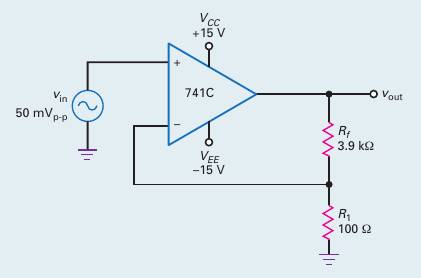
\includegraphics[width=1\linewidth]{gambar/fig-17.04}
		\end{center}
		\columnbreak
		\begin{itemize}
			\item Pertanyaan:
			\begin{itemize}
				\item Berdasarkan gambar di samping, jika $ A_{VOL} $ dari 741C adalah 100000, tentukan feedback fraction, ideal closed-loop voltage gain, percent error, dan exact closed-loop voltage gain.
			\end{itemize}
		\end{itemize}
	\end{multicols}
\end{frame}